\begin{frame}{Parallel specifications - example}
    \begin{figure}
        \centering
        \begin{tikzpicture}
        \useasboundingbox (0,0) rectangle (10,7.5);
        %\draw [blue!30,dotted] (current bounding box.north west) rectangle (current bounding box.south east);
        \draw [black,opacity=0] (5,0) -- (5,7.5);
        \end{tikzpicture}
        \caption{Two parallel specifications.}
    \end{figure}
    \begin{tikzpicture}[remember picture,overlay]
        \node[at=(current page.center),yshift=-0.2cm,xshift=-(\paperwidth+1cm)*0.26]{{

\newcommand{\tone}{%
\begin{tikzpicture}[scale=0.25, every node/.style={scale=0.25}, baseline=(current bounding box.center)]
\def\xscale{1} % Horizontal scale factor
\def\yscale{1} % Vertical scale factor
\def\spnt{0.15} % Size of smaller points
\def\lpnt{0.125} % Size of larger points
\draw (3.52*\xscale, 3.76*\yscale) -- (3.52*\xscale, 0);
\useasboundingbox (0,0) rectangle (7.04*\xscale,3.76*\yscale);
\draw[rounded corners=2ex*0.25] (0,0) rectangle (7.04*\xscale,3.76*\yscale);
\fill[red] (4.55*\xscale, 1.18*\yscale) circle (\spnt);
\fill[red] (6.05*\xscale, 2.78*\yscale) circle (\spnt);
\draw[red] (4.55*\xscale, 1.18*\yscale) -- (6.05*\xscale,2.78*\yscale);
\fill[red] (4.55*\xscale, 2.79*\yscale) circle (\spnt);
\fill[red] (6.05*\xscale, 1.12*\yscale) circle (\spnt);
\draw[red] (4.55*\xscale, 2.79*\yscale) -- (6.05*\xscale,1.12*\yscale);
\fill[red] (2.67*\xscale, 3.21*\yscale) circle (\spnt);
\fill[red] (4.29*\xscale, 0.3*\yscale) circle (\spnt);
\draw[red] (2.67*\xscale, 3.21*\yscale) -- (4.29*\xscale,0.3*\yscale);
\fill[red] (1.09*\xscale, 3.07*\yscale) circle (\spnt);
\fill[red] (1.526001050877835*\xscale, 3.393088634545991*\yscale) circle (\spnt);
\fill[red] (2.13*\xscale, 2.55*\yscale) circle (\spnt);
\draw[red] (1.09*\xscale, 3.07*\yscale) -- (1.526001050877835*\xscale,3.393088634545991*\yscale) -- (2.13*\xscale,2.55*\yscale);
\fill[red] (0.64*\xscale, 1.39*\yscale) circle (\spnt);
\fill[red] (1.01*\xscale, 0.79*\yscale) circle (\spnt);
\fill[red] (1.35*\xscale, 1.03*\yscale) circle (\spnt);
\draw[red] (0.64*\xscale, 1.39*\yscale) -- (1.01*\xscale,0.79*\yscale) -- (1.35*\xscale,1.03*\yscale);
\fill[red] (1.98*\xscale, 1.84*\yscale) circle (\spnt);
\fill[red] (2.3511520552717013*\xscale, 1.3932029657051672*\yscale) circle (\spnt);
\fill[red] (2.71*\xscale, 0.92*\yscale) circle (\spnt);
\draw[red] (1.98*\xscale, 1.84*\yscale) -- (2.3511520552717013*\xscale,1.3932029657051672*\yscale) -- (2.71*\xscale,0.92*\yscale);
\end{tikzpicture} 
}

\newcommand{\ttwo}{%
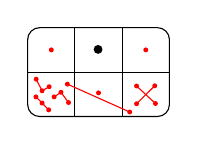
\begin{tikzpicture}[scale=0.3, every node/.style={scale=0.3}, baseline=(current bounding box.center)]
\def\xscale{1.0} % Horizontal scale factor
\def\yscale{1.0} % Vertical scale factor
\def\spnt{0.075*1.4} % Size of smaller points
\def\lpnt{0.125*1.5} % Size of larger points
\useasboundingbox (0,0) rectangle (6*\xscale,3.76*\yscale);
\draw[rounded corners=2ex*0.5] (0,0) rectangle (6*\xscale,3.76*\yscale);
\draw (2.0*\xscale, 3.76*\yscale) -- (2.0*\xscale, 0);
\draw (4.0*\xscale, 3.76*\yscale) -- (4.0*\xscale, 0);
\draw (0, 1.88*\yscale) -- (6.0*\xscale, 1.88*\yscale);
\fill[red] (4.61*\xscale, 0.54*\yscale) circle (\spnt);
\fill[red] (5.38*\xscale, 1.3*\yscale) circle (\spnt);
\draw[red] (4.61*\xscale, 0.54*\yscale) -- (5.38*\xscale,1.3*\yscale);
\fill[red] (1.68*\xscale, 1.37*\yscale) circle (\spnt);
\fill[red] (4.32*\xscale, 0.19*\yscale) circle (\spnt);
\draw[red] (1.68*\xscale, 1.37*\yscale) -- (4.32*\xscale,0.19*\yscale);
\fill[red] (4.61*\xscale, 1.29*\yscale) circle (\spnt);
\fill[red] (5.41*\xscale, 0.55*\yscale) circle (\spnt);
\draw[red] (4.61*\xscale, 1.29*\yscale) -- (5.41*\xscale,0.55*\yscale);
\fill[red] (1.12*\xscale, 0.83*\yscale) circle (\spnt);
\fill[red] (1.4096601986560762*\xscale, 1.0249991174784614*\yscale) circle (\spnt);
\fill[red] (1.73*\xscale, 0.59*\yscale) circle (\spnt);
\draw[red] (1.12*\xscale, 0.83*\yscale) -- (1.4096601986560762*\xscale,1.0249991174784614*\yscale) -- (1.73*\xscale,0.59*\yscale);
\fill[red] (1*\xscale, 2.82*\yscale) circle (\spnt);
\fill[red] (5*\xscale, 2.82*\yscale) circle (\spnt);
\fill[red] (3*\xscale, 1*\yscale) circle (\spnt);
\fill[red] (0.36*\xscale, 1.58*\yscale) circle (\spnt);
\fill[red] (0.6091281492290661*\xscale, 1.0877096738635244*\yscale) circle (\spnt);
\fill[red] (0.91*\xscale, 1.26*\yscale) circle (\spnt);
\draw[red] (0.36*\xscale, 1.58*\yscale) -- (0.6091281492290661*\xscale,1.0877096738635244*\yscale) -- (0.91*\xscale,1.26*\yscale);
\fill[red] (0.35*\xscale, 0.83*\yscale) circle (\spnt);
\fill[red] (0.61*\xscale, 0.57*\yscale) circle (\spnt);
\fill[red] (0.89*\xscale, 0.28*\yscale) circle (\spnt);
\draw[red] (0.35*\xscale, 0.83*\yscale) -- (0.61*\xscale,0.57*\yscale) -- (0.89*\xscale,0.28*\yscale);
\fill (2.98*\xscale,2.84*\yscale) circle (\lpnt);
\end{tikzpicture}
}

\newcommand{\tthree}{%
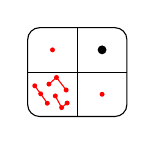
\begin{tikzpicture}[scale=0.3, every node/.style={scale=0.3}, baseline=(current bounding box.center)]
\def\xscale{1.0} % Horizontal scale factor
\def\yscale{1.0} % Vertical scale factor
\def\spnt{0.075*1.4} % Size of smaller points
\def\lpnt{0.125*1.5} % Size of larger points
\useasboundingbox (0,0) rectangle (4.2*\xscale,3.76*\yscale);
\draw[rounded corners=2ex*0.5] (0,0) rectangle (4.2*\xscale,3.76*\yscale);
\draw (2.1*\xscale, 3.76*\yscale) -- (2.1*\xscale, 0);
\draw (0, 1.88*\yscale) -- (4.2*\xscale, 1.88*\yscale);
\fill[red] (1.05*\xscale, 2.82*\yscale) circle (\spnt);
\fill[red] (3.15*\xscale, 0.94*\yscale) circle (\spnt);
\fill[red] (0.9*\xscale, 1.37*\yscale) circle (\spnt);
\fill[red] (1.2199471753311761*\xscale, 1.6524363073940609*\yscale) circle (\spnt);
\fill[red] (1.63*\xscale, 1.12*\yscale) circle (\spnt);
\draw[red] (0.9*\xscale, 1.37*\yscale) -- (1.2199471753311761*\xscale,1.6524363073940609*\yscale) -- (1.63*\xscale,1.12*\yscale);
\fill[red] (1.17*\xscale, 0.87*\yscale) circle (\spnt);
\fill[red] (1.436829177631258*\xscale, 0.37686266458866924*\yscale) circle (\spnt);
\fill[red] (1.67*\xscale, 0.57*\yscale) circle (\spnt);
\draw[red] (1.17*\xscale, 0.87*\yscale) -- (1.436829177631258*\xscale,0.37686266458866924*\yscale) -- (1.67*\xscale,0.57*\yscale);
\fill[red] (0.3*\xscale, 1.3*\yscale) circle (\spnt);
\fill[red] (0.55*\xscale, 0.96*\yscale) circle (\spnt);
\fill[red] (0.83*\xscale, 0.56*\yscale) circle (\spnt);
\draw[red] (0.3*\xscale, 1.3*\yscale) -- (0.55*\xscale,0.96*\yscale) -- (0.83*\xscale,0.56*\yscale);
\fill (3.150000000000005*\xscale,2.8210223642172525*\yscale) circle (\lpnt);
\end{tikzpicture}
}

\newcommand{\tfour}{%
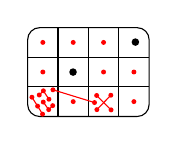
\begin{tikzpicture}[scale=0.3, every node/.style={scale=0.3}, baseline=(current bounding box.center)]
\def\xscale{1.0} % Horizontal scale factor
\def\yscale{1.0} % Vertical scale factor
\def\spnt{0.075*1.4} % Size of smaller points
\def\lpnt{0.16} % Size of larger points
\useasboundingbox (0,0) rectangle (5.14*\xscale,3.76*\yscale);
\draw[rounded corners=2ex*0.5] (0,0) rectangle (5.14*\xscale,3.76*\yscale);
\draw (1.285*\xscale, 3.76*\yscale) -- (1.285*\xscale, 0);
\draw (2.57*\xscale, 3.76*\yscale) -- (2.57*\xscale, 0);
\draw (3.855*\xscale, 3.76*\yscale) -- (3.855*\xscale, 0);
\draw (0, 1.2533333333333332*\yscale) -- (5.14*\xscale, 1.2533333333333332*\yscale);
\draw (0, 2.5066666666666664*\yscale) -- (5.14*\xscale, 2.5066666666666664*\yscale);
\fill[red] ({(0*1.285+0.6425)*\xscale}, {(1*1.253+0.63)*\yscale}) circle (\spnt);
\fill[red] ({(0*1.285+0.6425)*\xscale}, {(2*1.253+0.63)*\yscale}) circle (\spnt);
\fill[red] ({(1*1.285+0.6425)*\xscale}, {(0*1.253+0.63)*\yscale}) circle (\spnt);
\fill[red] ({(1*1.285+0.6425)*\xscale}, {(2*1.253+0.63)*\yscale}) circle (\spnt);
\fill[red] ({(2*1.285+0.6425)*\xscale}, {(1*1.253+0.63)*\yscale}) circle (\spnt);
\fill[red] ({(2*1.285+0.6425)*\xscale}, {(2*1.253+0.63)*\yscale}) circle (\spnt);
\fill[red] ({(3*1.285+0.6425)*\xscale}, {(0*1.253+0.63)*\yscale}) circle (\spnt);
\fill[red] ({(3*1.285+0.6425)*\xscale}, {(1*1.253+0.63)*\yscale}) circle (\spnt);
\fill[red] (2.93*\xscale, 0.29*\yscale) circle (\spnt);
\fill[red] (3.52*\xscale, 0.9*\yscale) circle (\spnt);
\draw[red] (2.93*\xscale, 0.29*\yscale) -- (3.52*\xscale,0.9*\yscale);
\fill[red] (1.07*\xscale, 1.13*\yscale) circle (\spnt);
\fill[red] (2.83*\xscale, 0.59*\yscale) circle (\spnt);
\draw[red] (1.07*\xscale, 1.13*\yscale) -- (2.83*\xscale,0.59*\yscale);
\fill[red] (2.92*\xscale, 0.89*\yscale) circle (\spnt);
\fill[red] (3.53*\xscale, 0.28*\yscale) circle (\spnt);
\draw[red] (2.92*\xscale, 0.89*\yscale) -- (3.53*\xscale,0.28*\yscale);
\fill[red] (0.49*\xscale, 0.91*\yscale) circle (\spnt);
\fill[red] (0.6644210751853692*\xscale, 1.086774200246225*\yscale) circle (\spnt);
\fill[red] (0.9*\xscale, 0.73*\yscale) circle (\spnt);
\draw[red] (0.49*\xscale, 0.91*\yscale) -- (0.6644210751853692*\xscale,1.086774200246225*\yscale) -- (0.9*\xscale,0.73*\yscale);
\fill[red] (0.66*\xscale, 0.61*\yscale) circle (\spnt);
\fill[red] (0.89*\xscale, 0.29*\yscale) circle (\spnt);
\fill[red] (1.06*\xscale, 0.46*\yscale) circle (\spnt);
\draw[red] (0.66*\xscale, 0.61*\yscale) -- (0.89*\xscale,0.29*\yscale) -- (1.06*\xscale,0.46*\yscale);
\fill[red] (0.18033887520734232*\xscale, 0.816133743581277*\yscale) circle (\spnt);
\fill[red] (0.42*\xscale, 0.44*\yscale) circle (\spnt);
\fill[red] (0.63*\xscale, 0.1*\yscale) circle (\spnt);
\draw[red] (0.18033887520734232*\xscale, 0.816133743581277*\yscale) -- (0.42*\xscale,0.44*\yscale) -- (0.63*\xscale,0.1*\yscale);
\fill (1.92*\xscale,1.88*\yscale) circle (\lpnt);
\fill (4.56*\xscale,3.15*\yscale) circle (\lpnt);
\end{tikzpicture}
}

\newcommand{\tpair}{%
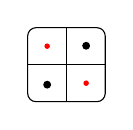
\begin{tikzpicture}[scale=0.25, every node/.style={scale=0.25}, baseline=(current bounding box.center)]
\def\xscale{1.0} % Horizontal scale factor
\def\yscale{1.0} % Vertical scale factor
\def\spnt{0.14} % Size of smaller points
\def\lpnt{0.2} % Size of larger points
\useasboundingbox (0,0) rectangle (3.94*\xscale,3.76*\yscale);
\draw[rounded corners=2ex*.35] (0,0) rectangle (3.94*\xscale,3.76*\yscale);
\draw (1.97*\xscale, 3.76*\yscale) -- (1.97*\xscale, 0);
\draw (0, 1.88*\yscale) -- (3.94*\xscale, 1.88*\yscale);
\fill (0.99*\xscale,0.864920127795527*\yscale) circle (\lpnt);
\fill (2.97*\xscale,2.841054313099042*\yscale) circle (\lpnt);
\fill[red] (0.99*\xscale,3.76*0.75*\yscale) circle (\spnt);
\fill[red] (3*0.99*\xscale,3.76*0.25*\yscale) circle (\spnt);
\end{tikzpicture}
}

\newcommand{\pntatom}{\tikz\fill (0,0) circle (0.1);}


\begin{tikzpicture}
    \draw [black,opacity=0] (-3.25,-6.87) rectangle (2.75,0.60);
    %\viewborder
    
    \node (rootB) at (0, 0) {\tone};
    
    \node<1,3-> (lvl11B) at (-1.5,-1.75) {\ttwo};
    \node<1,3-6,12-> (lvl12B) at (0,-1.75) {$\varepsilon$};
    \node<1,3-6,13-> (lvl13B) at (1.5,-1.75) {\tthree};
    \draw<1,3->\ptedge{(rootB.south)}{(-0.5,1.4)}{(lvl11B)}{(-0.5,0.9)};
    \draw<1,3-6,12->\ptedge{(rootB.south)}{(-0.5,1.4)}{(lvl12B)}{(-0.5,0.5)};
    \draw<1,3-6,13->\ptedge{(rootB.south)}{(-0.5,1.4)}{(lvl13B)}{(-0.5,0.9)};
    \circover{0,-.725}{0.13}{\tiny $\sqcup$}{1,3-}
    
    % Bijection greens and eq examples
    \draw<4>[orange] (lvl11B.south west) rectangle (lvl13B.north east);
    \draw<5> (-1.5, -3.5) node {$\mathcal{A}$};
    \draw<5> (lvl11B.south) -- (-1.5,-3.25);
    \draw<5> (-1.5, -5) node {$\mathcal{B}$};
    \draw<5> (-1.5,-3.75) -- (-1.5,-4.75);
    \draw<5> (1.5, -3.5) node {$\mathcal{C}$};
    \draw<5> (lvl13B.south) -- (1.5,-3.25);
    \draw<5> [orange] (-1.5-0.25,-5-0.25) rectangle (-1.5+.25,-5+.25);
    \draw<5> [orange] (1.5-0.25,-3.5-0.25) rectangle (1.5+.25,-3.5+.25);
    \draw<5> [orange] (0-.25,-1.75-.2) rectangle (0+.25,-1.75+.2);
    \circover{-1.5,-2.65}{0.13}{\tiny $\cong$}{5}
    \circover{-1.5,-3.95}{0.13}{\tiny $\cong$}{5}
    \circover{1.5,-2.65}{0.13}{\tiny $\cong$}{5}
    
    \node<1,7-> (lvl21B) at (-2.25,-3.5) {\tone};
    \coordinate (lvl22Bphantom) at (-0.75,-3.15);
    \node<1,7-> (lvl22B) at (-0.75,-3.5) {\pntatom};
    \draw<1,7->\ptedge{(lvl11B.south)}{(-0.5,1.4)}{(lvl21B)}{(-0.5,0.8)};
    \draw<1,7->\ptedge{(lvl11B.south)}{(-0.5,1.4)}{(lvl22Bphantom)}{(-0.5,0.45)};
    \draw<1,7-> ([yshift=0.18cm]lvl22Bphantom) -- (lvl22B);
    \circover{-1.5,-2.6}{0.13}{\tiny $\times$}{1,7-}
    
    \node<1,13-> (lvl23B) at (0.75,-3.5) {\tfour};
    \coordinate (lvl24Bphantom) at (2.25,-3.05);
    \node<1,13-> (lvl24B) at (2.25,-3.5) {\pntatom};
    \draw<1,13->\ptedge{(lvl13B.south)}{(-0.5,1.4)}{(lvl23B)}{(-0.5,0.89)};
    \draw<1,13->\ptedge{(lvl13B.south)}{(-0.5,1.4)}{(lvl24Bphantom)}{(-0.5,0.45)};
    \draw<1,13-> ([yshift=0.145cm]lvl24Bphantom) -- (lvl24B);
    \circover{1.5,-2.6}{0.13}{\tiny $\sqcup$}{1,13-}
    
    \node<1,14-> (lvl31B) at (0.75-1,-5.25) {\tpair};
    \node<1,14-> (lvl32B) at (0.75+1,-5.25) {\tone};
    \draw<1,14->\ptedge{(lvl23B.south)}{(-0.5,1.4)}{(lvl31B)}{(-0.5,0.8)};
    \draw<1,14->\ptedge{(lvl23B.south)}{(-0.5,1.4)}{(lvl32B)}{(-0.5,0.8)};
    \circover{0.75,-4.34}{0.13}{\tiny $\times$}{1,14-}
    
    \node<1,15-> (lvl41B) at (-1.25,-7+.35) {\pntatom};
    \node<1,15-> (lvl42B) at (0.75,-7+.35) {\pntatom};
    \draw<1,15->\ptedge{(lvl31B.south)}{(-0.5,1.4)}{(lvl41B)}{(-0.5,0.475)};
    \draw<1,15->\ptedge{(lvl31B.south)}{(-0.5,1.4)}{(lvl42B)}{(-0.5,0.475)};
    \circover{-.25,-6}{0.13}{\tiny $\times$}{1,15-}
\end{tikzpicture}
}};
    \end{tikzpicture}
    \begin{tikzpicture}[remember picture,overlay]
        \node[at=(current page.center),yshift=-0.2cm,xshift=(\paperwidth-1cm)*0.26]{{

\newcommand{\binroot}{(0\,|\,10)\!\ast(1\,|\,\varepsilon)}

\newcommand{\binsize}{\fontsize{7pt}{7pt}}

\begin{tikzpicture}
    \draw [black,opacity=0]  (-3.2,-6.87) rectangle (2.8,0.60);
    %\viewborder
    
    \node (rootA) at (0,0) {\binsize$\binroot$};
    
    \node<1,3-7,13-> (lvl11A) at (-1.75,-1.75) {\binsize$1|(01\binroot)$};
    \node<1,3-6,8,12-> (lvl12A) at (0,-1.75) {\binsize$\varepsilon$};
    \node<1,3-6,9-> (lvl13A) at (1.25,-1.75) {\binsize$0\binroot$};
    \draw<1,3-7,13->\ptedge{(rootA.south)}{(-0.5,1.4)}{(lvl11A)}{(0,0.55)};
    \draw<1,3-6,8,12->\ptedge{(rootA.south)}{(-0.5,1.4)}{(lvl12A)}{(-0.5,0.55)};
    \draw<1,3-6,9->\ptedge{(rootA.south)}{(-0.5,1.4)}{(lvl13A)}{(-0.5,0.55)};
    \circover{0,-0.4}{0.13}{\tiny $\sqcup$}{1,3-}
    
    \draw<4>[orange] (lvl11A.south west) rectangle (lvl13A.north east);
    
    \draw<5> (-1.75, -3.5) node {$\mathcal{D}$};
    \draw<5> (lvl11A.south) -- (-1.75,-3.25);
    \circover{-1.75,-2.2}{0.13}{\tiny $\cong$}{5}
    \draw<5> [orange] (-1.75-0.25,-3.5-0.25) rectangle (-1.75+.25,-3.5+.25);
    \draw<5>[orange] ([yshift=-0.05cm,xshift=-.05cm]lvl12A.south west) rectangle (lvl13A.north east);
    
    \node<1,7,13-> (lvl21A) at (-1.75-0.75,-3.5) {\binsize$1$};
    \node<1,7,13-> (lvl22A) at (-1.75+0.75,-3.5) {\binsize$10\binroot$};
    \draw<1,7,13->\ptedge{(lvl11A.south)}{(-0.5,1.4)}{(lvl21A)}{(-0.5,0.55)};
    \draw<1,7,13->\ptedge{(lvl11A.south)}{(-0.5,1.4)}{(lvl22A)}{(-0.5,0.55)};
    \circover{-1.75,-2.15}{0.13}{\tiny $\sqcup$}{1,7,13-}
    
    \node<1,9-> (lvl23A) at (1.25-0.6,-3.5) {\binsize$0$};
    \node<1,9,11-> (lvl24A) at (1.25+0.6,-3.5) {\binsize$\binroot$};
    \draw<10> (1.25+0.6,-3.5) node {$\mathcal{A}$};
    \draw<10>[-] (1.25+0.6,-3.8) -- (1.25+0.6,-4.8);
    \circover{1.25+0.6,-4.05}{0.13}{\tiny $\cong$}{10}
    \draw<10> (1.25+0.6,-5) node {\binsize$\binroot$};
    
    \draw<1,9->\ptedge{(lvl13A.south)}{(-0.5,1.4)}{(lvl23A)}{(-0.5,0.55)};
    \draw<1,9->\ptedge{(lvl13A.south)}{(-0.5,1.4)}{(lvl24A)}{(-0.5,0.55)};
    \circover{1.25,-2.15}{0.13}{\tiny $\times$}{1,9-}
    
    \node<1,14-> (lvl31A) at (-1.75+0.75-1,-5.25) {\binsize$10$};
    \node<1,14-> (lvl32A) at (-1.75+0.75+1,-5.25) {\binsize$\binroot$};
    \draw<1,14->\ptedge{(lvl22A.south)}{(-0.5,1.4)}{(lvl31A)}{(-0.5,0.55)};
    \draw<1,14->\ptedge{(lvl22A.south)}{(-0.5,1.4)}{(lvl32A)}{(-0.5,0.55)};
    \circover{-1,-3.9}{0.13}{\tiny $\times$}{1,14-}
    
    \node<1,15-> (lvl41A) at (-1.75+0.75-1-.95,-7+.35) {\binsize$1$};
    \node<1,15-> (lvl42A) at (-1.75+0.75-1+.95,-7+.35) {\binsize$0$};
    \draw<1,15->\ptedge{(lvl31A.south)}{(-0.5,1.4)}{(lvl41A)}{(-0.5,0.55)};
    \draw<1,15->\ptedge{(lvl31A.south)}{(-0.5,1.4)}{(lvl42A)}{(-0.5,0.55)};
    \circover{-2,-5.625}{0.13}{\tiny $\times$}{1,15-}
\end{tikzpicture}
}};
    \end{tikzpicture}
\end{frame}